\section{整性}\label{sec:integrality}

考虑环的包含 $R\subseteq S$, 并把 $S$ 看作 $R$-模. 在什么条件下, $S$ 是有限生成 $R$-模? 上一节末研究了两种这样的情形:
\begin{enumerate}
  \item $R=\mathbb{Z}$ 且 $S=\mathbb{Z}[\sqrt{2}]$;
  \item $R=\mathbb{Z}$ 且 $S=\mathbb{Z}[1/2]$.
\end{enumerate}
在第一种情形中, 我们看到 $\mathbb{Z}[\sqrt{2}]$ 确实是有限生成 $\mathbb{Z}$-模. 在第二种情形中, 我们论证了 $\mathbb{Z}[1/2]$ 不是. 回顾这些例子, $\sqrt{2}$ 和 $1/2$ 的一个主要区别是: 对 $\sqrt{2}$ 取幂最终会得到 $\mathbb{Z}$ 中的元素, 而对 $1/2$ 取幂则始终回不到 $\mathbb{Z}$. 正是 $(\sqrt{2})^{2}=2$ 这一事实, 使我们能把所有关于 $\sqrt{2}$ 的多项式表达式化为一次多项式.

本节的目标是将以上观察推广到一般的环, 并给出准确的表述. 这里关键的新概念是\emph{整性}. 为引出下面的定义, 回忆首一多项式是首项系数为 $1$ 的非零多项式. 也就是说, $R[x]$ 中的首一多项式形如
\[
  x^{n}+a_{n-1}x^{n-1}+\cdots+a_{1}x+a_{0},
\]
其中 $n\geq0$, $a_{0},\ldots,a_{n-1}\in R$.

\begin{Definition}{代数元与整元}\leavevmode\label{def:algebraic-and-integral-elements}
  设 $R\subseteq S$ 为环, $a\in S$. 若存在非零多项式 $f\in R[x]$ 使得 $f(a)=0\in S$, 则称 $a$ \textbf{在 $R$ 上代数}. 进一步, 若存在首一多项式 $f\in R[x]$ 使得 $f(a)=0$, 则称 $a$ \textbf{在 $R$ 上整}.
\end{Definition}

若 $R$ 是域, 一个元素是代数元当且仅当它是整元, 因为可以用任意非零多项式除以其首项系数来得到首一多项式. 在更一般的环中, 除法未必有意义, 因此整性比代数性更强.

在 $R=\mathbb{Z}$ 且 $S=\mathbb{R}$ 的情形下看几个例子.

\begin{Example}{$\sqrt{2}$ 在 $\mathbb{Z}$ 上整}\leavevmode\label{ex:square-root-two-integral}
  因为 $a=\sqrt{2}$ 是首一多项式
  \[
    x^{2}-2\in\mathbb{Z}[x]
  \]
  的一个根, 所以 $\sqrt{2}$ 在 $\mathbb{Z}$ 上整.
\end{Example}

\begin{Example}{$\pi$ 在 $\mathbb{Z}$ 上不是代数元}\leavevmode\label{ex:pi-not-algebraic}
  在学习数学的某个阶段, 你或许知道了 $\pi$ 是超越数. 这就是说它不满足 $\mathbb{Z}$ 上的任何多项式方程. 因而 $\pi$ 在 $\mathbb{Z}$ 上不是代数元.
\end{Example}

\begin{Example}{$1/2$ 在 $\mathbb{Z}$ 上代数但不整}\leavevmode\label{ex:half-algebraic-not-integral}
  元素 $a=1/2$ 在 $\mathbb{Z}$ 上代数, 因为它是多项式
  \[
    g(x)=2x-1\in\mathbb{Z}[x]
  \]
  的一个根, 但它不整. 这一点并非显而易见: 虽然 $g$ 不是首一的, 但也许仍会希望存在以 $1/2$ 为根的首一多项式. 然而, 如果
  \[
    h(x)=x^{n}+a_{n-1}x^{n-1}+\cdots+a_{1}x+a_{0}\in\mathbb{Z}[x]
  \]
  是这样的多项式, 那么将等式 $h(1/2)=0$ 的两边乘以 $2^{n-1}$, 得
  \[
    \frac{1}{2}+a_{n-1}+a_{n-2}\cdot2+a_{n-3}\cdot2^{2}
      +\cdots+a_{1}\cdot2^{n-2}+a_{0}\cdot2^{n-1}=0.
  \]
  \BookPairedNote
    {把第一项以外的项都移到右边, 就把 $1/2$ 表示成了整数之和. 这是不可能的, 所以 $1/2$ 不整.}
    {更一般地, 有理数 $a\in\mathbb{Q}$ 在 $\mathbb{Z}$ 上整当且仅当 $a\in\mathbb{Z}$ (Exercise~\ref{ex:rational-integral-iff-integer}).}
\end{Example}

$S$ 的每个元素都有可能在 $R$ 上代数, 甚至都在 $R$ 上整. 此时使用以下术语.

\begin{Definition}{代数扩张与整扩张}\leavevmode\label{def:algebraic-and-integral-extensions}
  设 $R\subseteq S$ 为环. 若 $S$ 的每个元素都在 $R$ 上代数 (分别地, 在 $R$ 上整), 则称 $S$ \textbf{是 $R$ 的代数扩张} (分别地, \textbf{是 $R$ 的整扩张}).
\end{Definition}

\begin{Example}{{\textmd{$\mathbb{Z}[\sqrt{2}]$} 在 $\mathbb{Z}$ 上整}}\leavevmode\label{ex:sqrt-two-ring-integral}
  要证明 $\mathbb{Z}[\sqrt{2}]$ 在 $\mathbb{Z}$ 上整, 必须说明 $\mathbb{Z}[\sqrt{2}]$ 的每个元素都在 $\mathbb{Z}$ 上整. 为此, 先回顾 (Example~\ref{ex:square-root-two-finite-module})
  \[
    \mathbb{Z}[\sqrt{2}]=\{r+s\sqrt{2}\mid r,s\in\mathbb{Z}\}.
  \]
  因此, 给定 $\mathbb{Z}[\sqrt{2}]$ 中一个元素, 可把它写成 $r+s\sqrt{2}$, 其中 $r,s\in\mathbb{Z}$. 平方后得到
  \[
    (r+s\sqrt{2})^{2}=(r^{2}+2s^{2})+(2rs)\sqrt{2}.
  \]
  移项后再次平方, 得
  \[
    \bigl((r+s\sqrt{2})^{2}-(r^{2}+2s^{2})\bigr)^{2}=(2rs)^{2}\cdot2.
  \]
  最后一个等式表明 $r+s\sqrt{2}$ 是四次首一多项式
  \[
    f(x)=\bigl(x^{2}-(r^{2}+2s^{2})\bigr)^{2}-(2rs)^{2}\cdot2\in\mathbb{Z}[x]
  \]
  的一个根. 因此 $\mathbb{Z}[\sqrt{2}]$ 的每个元素都在 $\mathbb{Z}$ 上整.
\end{Example}

\begin{Example}{$\mathbb{R}$ 不是 $\mathbb{Z}$ 的代数扩张}\leavevmode\label{ex:reals-not-algebraic-over-integers}
  因为实数中含有超越数, 如 $\pi$, 所以 $\mathbb{R}$ 不是 $\mathbb{Z}$ 的代数扩张.
\end{Example}

\begin{Example}{$\mathbb{Q}$ 是 $\mathbb{Z}$ 的代数扩张, 但不是整扩张}\leavevmode\label{ex:rationals-algebraic-not-integral}
  环 $\mathbb{Q}$ 是 $\mathbb{Z}$ 的代数扩张, 因为 $a=p/q\in\mathbb{Q}$ 是多项式 $f(x)=qx-p\in\mathbb{Z}[x]$ 的一个根. 但由 Example~\ref{ex:half-algebraic-not-integral}, $\mathbb{Q}$ 不是 $\mathbb{Z}$ 的整扩张.
\end{Example}

现在回到我们的目标: 判定有限生成 $R$-代数何时作为 $R$-模也是有限生成的. 这与整性密切相关. 具体来说, 下面的结果告诉我们, 一个有限生成 $R$-代数是有限生成 $R$-模, 当且仅当它在 $R$ 上整. 此外, 为验证整性, 只须验证各代数生成元在 $R$ 上整.

\begin{Theorem}{有限生成与整性}\leavevmode\label{thm:finite-generation-integrality}
  设 $R\subseteq S$ 为环, 且 $S=R[a_{1},\ldots,a_{n}]$. 下列条件等价:
  \begin{enumerate}[label=(\roman*)]
    \item $S$ 是有限生成 $R$-模;
    \item $S$ 在 $R$ 上整;
    \item 对每个 $i=1,\ldots,n$, $a_{i}$ 均在 $R$ 上整.
  \end{enumerate}
\end{Theorem}

在开始证明前, 先指出论证将涉及一些矩阵运算, 这些矩阵的元素来自环 $R$, 而读者可能还未在这么一般的情形中处理过矩阵. 所有这类运算, 如矩阵与向量相乘或矩阵的行列式, 都用与较熟悉的实数或其他域上相同的公式定义. 这些定义对任意环中的元素都有意义, 因为只涉及元素的和与积.

\begin{Proof}\textbf{of Theorem~\ref{thm:finite-generation-integrality}.}\quad
  证明 (i) $\Rightarrow$ (ii) $\Rightarrow$ (iii) $\Rightarrow$ (i).

  \textbf{(i)} $\Rightarrow$ \textbf{(ii):} 假设 $S$ 是有限生成 $R$-模. 这意味着存在 $v_{1},\ldots,v_{m}\in S$, 使得 $S=R\{v_{1},\ldots,v_{m}\}$. 必须证明任意元素 $b\in S$ 都在 $R$ 上整. 为此, 先将 $b$ 乘以每个模生成元, 并将乘积写成这些生成元的线性组合:
  \[
    bv_{i}=c_{i1}v_{1}+c_{i2}v_{2}+\cdots+c_{im}v_{m},
  \]
  其中 $i,j=1,\ldots,m$ 时 $c_{ij}\in R$. 将每个等式的所有项移到左边, 得线性方程组
  \[
    \begin{aligned}
      (b-c_{11})v_{1}+(-c_{12})v_{2}+\cdots+(-c_{1m})v_{m}&=0\\
      (-c_{21})v_{1}+(b-c_{22})v_{2}+\cdots+(-c_{2m})v_{m}&=0\\
      &\ \vdots\\
      (-c_{m1})v_{1}+(-c_{m2})v_{2}+\cdots+(b-c_{mm})v_{m}&=0.
    \end{aligned}
  \]
  这样的方程组写成矩阵与向量相乘更方便: 若 $C$ 是第 $(i,j)$ 个元素为 $c_{ij}$ 的矩阵, 则
  \begin{equation}\label{eq:module-generators-matrix-system}
    (bI-C)\cdot
    \begin{pmatrix}v_{1}\\\vdots\\v_{m}\end{pmatrix}
    =\begin{pmatrix}0\\\vdots\\0\end{pmatrix},
  \end{equation}
  其中 $I$ 是 $m\times m$ 单位矩阵.

  此时用到 Cramer 法则, 读者在学习线性代数时可能见过这一关于矩阵的结果. 这里先给出其表述, 证明见 Exercise~\ref{ex:determinant-cramer-rule}.

  \begin{Lemma}{Cramer 法则}\leavevmode\label{lem:cramers-rule-over-ring}
    设 $A$ 是元素在环 $R$ 中的 $m\times m$ 矩阵. 设 $v,w\in R^{m}$, 将它们看作列向量, 并假设
    \[
      Av=w.
    \]
    则对所有 $i=1,\ldots,m$,
    \[
      \det(A)\cdot v_{i}=\det(A_{i}),
    \]
    其中 $A_{i}$ 由 $A$ 将第 $i$ 列替换为 $w$ 而得到.
  \end{Lemma}

  将这个工具应用于矩阵等式 \eqref{eq:module-generators-matrix-system}, 得到
  \begin{equation}\label{eq:determinant-annihilates-module-generators}
    \det(bI-C)\cdot v_{i}=0
  \end{equation}
  对所有 $i$ 成立. 注意, 右边为零是因为它是一个有一列全为零的矩阵的行列式. 回顾 $v_{i}$ 是 $S$ 作为 $R$-模的生成元, 故可将 $1\in S$ 表示成 $v_{1},\ldots,v_{m}$ 的线性组合:
  \[
    1=d_{1}v_{1}+\cdots+d_{m}v_{m}.
  \]
  两边乘以 $\det(bI-C)$ 并应用 \eqref{eq:determinant-annihilates-module-generators}, 得
  \[
    \det(bI-C)=0.
  \]
  因此 $b$ 是多项式
  \[
    f(x)=\det(xI-C)\in R[x]
  \]
  的一个根. 由行列式的性质, $f(x)=\det(xI-C)$ 作为 $x$ 的多项式, 其首项正是对角元素乘积的首项:
  \[
    f(x)=\prod_{i=1}^{m}(x-c_{ii})+\text{关于 $x$ 的次数至多为 $m-1$ 的各项}.
  \]
  从而 $f(x)$ 首一, 这证明了 $b$ 在 $R$ 上整.

  \textbf{(ii)} $\Rightarrow$ \textbf{(iii):} 若 $S$ 在 $R$ 上整, 则 $S$ 的每个元素都在 $R$ 上整, 所以每个 $a_{i}$ 都整.

  \textbf{(iii)} $\Rightarrow$ \textbf{(i):} 假设各 $a_{i}$ 都在 $R$ 上整, 则存在首一多项式 $f_{1},\ldots,f_{n}\in R[x]$, 使每个 $f_{i}(a_{i})=0$. 以 $d_{i}>0$ 记 $f_{i}$ 的次数. 我们要证明 $S$ 作为 $R$-模由有限集
  \[
    \mathcal{T}=\{a_{1}^{k_{1}}\cdots a_{n}^{k_{n}}\mid 0\leq k_{i}<d_{i}\}
  \]
  生成. 证明 $S=R\mathcal{T}$ 的第一步是, 对每个 $i=1,\ldots,n$ 证明
  \begin{equation}\label{eq:single-integral-element-module-span}
    R[a_{i}]=R\{a_{i}^{k_{i}}\mid 0\leq k_{i}<d_{i}\}.
  \end{equation}
  这一步通过归纳论证得到: 利用关系 $f_{i}(a_{i})=0$ 降低关于 $a_{i}$ 的多项式表达式的次数 (Exercise~\ref{ex:monic-relation-bounds-module-powers}), 类似于在 Example~\ref{ex:square-root-two-finite-module} 中论证 $\mathbb{Z}[\sqrt{2}]=\mathbb{Z}\{1,\sqrt{2}\}$ 的办法. 一旦确立 \eqref{eq:single-integral-element-module-span}, 对任意 $\ell_{i}\geq0$, 就能把 $a_{i}^{\ell_{i}}\in R[a_{i}]$ 写成 $\{a_{i}^{k_{i}}\mid 0\leq k_{i}<d_{i}\}$ 的 $R$-线性组合. 将这些线性组合相乘并展开, 可知对任意 $\ell_{1},\ldots,\ell_{n}\geq0$, 元素
  \begin{equation}\label{eq:products-of-arbitrary-powers}
    a_{1}^{\ell_{1}}\cdots a_{n}^{\ell_{n}}\in S
  \end{equation}
  都可写成 $\mathcal{T}$ 中元素的 $R$-线性组合.

  因为 $S=R[a_{1},\ldots,a_{n}]$ 的每个元素都可写成形如 \eqref{eq:products-of-arbitrary-powers} 且 $\ell_{1},\ldots,\ell_{n}\geq0$ 的表达式的 $R$-线性组合, 而每个这样的表达式 \eqref{eq:products-of-arbitrary-powers} 又可写成 $\mathcal{T}$ 中元素的 $R$-线性组合, 所以 $S$ 的每个元素都可写成 $\mathcal{T}$ 中元素的 $R$-线性组合. 这正好证明了 $S=R\mathcal{T}$.
\end{Proof}

一般而言, 给定环扩张 $R\subseteq S$, 环 $S$ 在 $R$ 上无论作为 $R$-模还是作为 $R$-代数都未必有限生成, 也未必在 $R$ 上整. 但是 Theorem~\ref{thm:finite-generation-integrality} 告诉我们, 既是有限生成 $R$-代数又在 $R$ 上整的那些扩张, 恰好就是有限生成 $R$-模. \hyperref[fig:integrality-venn-diagram]{下方的 Venn 图}说明了这一结果.

\par\smallskip
{\centering
\begin{tikzpicture}
  \phantomsection\label{fig:integrality-venn-diagram}
  \node[inner sep=0pt,anchor=south west] (venn) at (0,0)
    {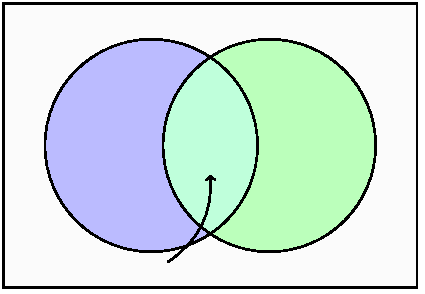
\includegraphics[width=.65\linewidth]{figures/integrality-venn-geometry.pdf}};
  \begin{scope}[x={(venn.south east)},y={(venn.north west)},every node/.style={font=\small,inner sep=0pt,align=center}]
    \node at (.50,.937) {包含 $R$ 的环};
    \node at (.251,.527) {有限生成\\$R$-代数};
    \node at (.755,.500) {$R$ 的整扩张};
    \node at (.386,.071) {有限生成 $R$-模};
  \end{scope}
\end{tikzpicture}\par}

\BookExerciseHeading
\begin{BookExercises}
  \item\label{ex:square-root-of-two-root-test} 元素 $\frac{\sqrt{2}}{2}\in\mathbb{R}$ 在 $\mathbb{Z}$ 上代数吗? 整吗?
  \item\label{ex:rational-integral-iff-integer} 证明 $a\in\mathbb{Q}$ 在 $\mathbb{Z}$ 上整当且仅当 $a\in\mathbb{Z}$. 这说明了\textquotedbl{}整\textquotedbl{}这个术语的由来.
  \item\label{ex:complex-integral-over-real} 证明 $\mathbb{C}$ 在 $\mathbb{R}$ 上整 (或等价地, 代数). (提示: 仿照 Example~\ref{ex:sqrt-two-ring-integral} 的论证.)
  \item\label{ex:classify-integral-polynomial-quotients} 对下列各环, 令 $a=[x]$ 为 $x$ 的陪集, 判定这个环是否在子环 $R[a]$ 上整.
    \begin{enumerate}[label=(\alph*)]
      \item $R[x,y]$
      \item $R[x,y]/\langle y^{2}-x^{2}\rangle$
      \item $R[x,y]/\langle xy\rangle$
      \item $R[x,y,z]/\langle y^{2}-x^{3},z^{3}-x^{4}\rangle$
    \end{enumerate}
  \item\label{ex:rationals-not-finite-module-direct} 由 Example~\ref{ex:rationals-algebraic-not-integral} 可知 $\mathbb{Q}$ 不在 $\mathbb{Z}$ 上整, 所以 Theorem~\ref{thm:finite-generation-integrality} 蕴含 $\mathbb{Q}$ 不是有限生成 $\mathbb{Z}$-模. 请直接验证这一点: 说明对于任意 $a_{1},\ldots,a_{n}\in\mathbb{Q}$, 都有真包含
    \[
      \mathbb{Z}\{a_{1},\ldots,a_{n}\}\subsetneq\mathbb{Q}.
    \]
  \item\label{ex:determinant-cramer-rule} 本题证明 Cramer 法则, 假定读者熟悉矩阵乘法和行列式. 设 $A$ 是元素在环 $R$ 中的 $m\times m$ 矩阵, 向量 $v,w\in R^{m}$ 满足 $Av=w$.
    \begin{enumerate}[label=(\alph*)]
      \item 以 $I_{i}$ 记由 $m\times m$ 单位矩阵 $I$ 将第 $i$ 列替换为 $v$ 而得的矩阵. 证明
        \[
          AI_{i}=A_{i},
        \]
        其中 $A_{i}$ 由 $A$ 将第 $i$ 列替换为 $w$ 而得到.
      \item 用你喜欢的求行列式的方法证明
        \[
          \det(I_{i})=v_{i},
        \]
        再利用行列式的乘法性得出
        \[
          \det(A)\cdot v_{i}=\det(A_{i}).
        \]
    \end{enumerate}
  \item\label{ex:monic-relation-bounds-module-powers} 设 $R\subseteq S$ 为环, $a\in S$. 假设存在 $d$ 次首一多项式 $f\in R[x]$ 使 $f(a)=0$. 证明
    \[
      R[a]=R\{1,a,a^{2},\ldots,a^{d-1}\}.
    \]
    若 $f$ 不首一, 你的证明会在哪一步失效?
  \item\label{ex:integral-closure-is-subring} 设 $R\subseteq S$ 为环. 证明集合 $\{s\in S\mid s\text{ 在 $R$ 上整}\}$ 是 $S$ 中包含 $R$ 的子环. (提示: 使用 Theorem~\ref{thm:finite-generation-integrality}.) 这个子环称为 $R$ 在 $S$ 中的整闭包.
  \item\label{ex:integrality-venn-regions} 令 $R=\mathbb{Z}$. 对本节 \hyperref[fig:integrality-venn-diagram]{Venn 图}中的每个区域, 描述位于该区域中的环 $S$ 的例子.
\end{BookExercises}
